ex
% This is LLNCS.DEM the demonstration file of
% the LaTeX macro package from Springer-Verlag
% for Lecture Notes in Computer Science,
% version 2.4 for LaTeX2e as of 16. April 2010
%
\documentclass{llncs}
%
\usepackage{makeidx}  % allows for indexgeneration
\usepackage[utf8]{inputenc}
\usepackage{graphicx}
\usepackage{algorithmic}
\usepackage{algorithm}
\usepackage{subfig}
\usepackage{float}
%\usepackage{hyperref}

%
\begin{document}
%
\frontmatter          % for the preliminaries
%
\pagestyle{headings}  % switches on printing of running heads
\addtocmark{Eternity II} % additional mark in the TOC
%

\mainmatter              % start of the contributions
%
\title{Solving Eternity II\\
    \small{An approach based on Genetic Algorithms}
  }
  %
  \titlerunning{Eternity II - Genetic Algorithms Approach}  % abbreviated title (for running head)
  %                                     also used for the TOC unless
  %                                     \toctitle is used
  %
  \author{João Gradim \and Mário Carneiro}
  %
  \authorrunning{João Gradim\inst{1} et Mário Carneiro\inst{1}} % abbreviated author list (for running head)
%
%%%% list of authors for the TOC (use if author list has to be modified)
\tocauthor{João Gradim and Mário Carneiro}
%
\institute{Faculdade de Engenharia da Universidade do Porto,\\
\email{ei05030@fe.up.pt}, \email{ei04051@fe.up.pt}}

\maketitle              % typeset the title of the contribution

\begin{abstract}
%TODO: o abstract escreve-se no fim.
Eternity II is an NP-complete edge-matching puzzle which solution has not yet been discovered. This article, we will describe how it is possible to tackle this problem by using genetic algorithms.
\end{abstract}
%
\section{Introduction}\label{sec:introduction}

The Eternity II puzzle is an edge-matching puzzle. It consists of a 16 by 16 grid that must be completed with the respective 256 pieces. Each piece has four coloured patterns on its edges. The tiles are placed on a 16x16 board and can be freely rotated before being placed.

A solution is found when all of the edges match their neighboring tiles' edges. The puzzle was conceived specifically so it is very difficult to solve by brute force searching methods. The puzzle was designed as a competition by Christopher Monckton in 2005. A two million US dollars prize is being offered to the first complete solution of this puzzle.

% TODO: cite http://www.prnewswire.co.uk/cgi/news/release?id=188486

Our work was toward solving smaller versions of this puzzle - with less edge patterns and a board of smaller dimensions.

We will also use an existing element to base our work upon: The \textit{Eternity II Editor} is an open-source Java-based application that allows the creation and edition of Eternity II puzzle grids. \textit{Eternity II Editor}'s features include a series of puzzle solving programs and the ability to see the program's attempt to solve the puzzle in real time. More importantly, it features a usable application interface that will allow us to extend the application with out own solving methods.

\section{Problem Description}\label{sec:problem_description}

\subsection{Eternity II puzzle description}\label{sec:puzzle_description}

The Eternity II puzzle is an edge-matching puzzle. Solving the puzzle means placing the puzzle's 256 square pieces on a 16 by 16  grid in such a way that all of the pieces' edges match adjacent edges. The puzzle was designed to be difficult to solve by brute-force computer search, as there are roughly $1.115 * 10 ^ {557}$ possible configurations.

\begin{figure}[H]
  \centering
  \subfloat[Shuffled]{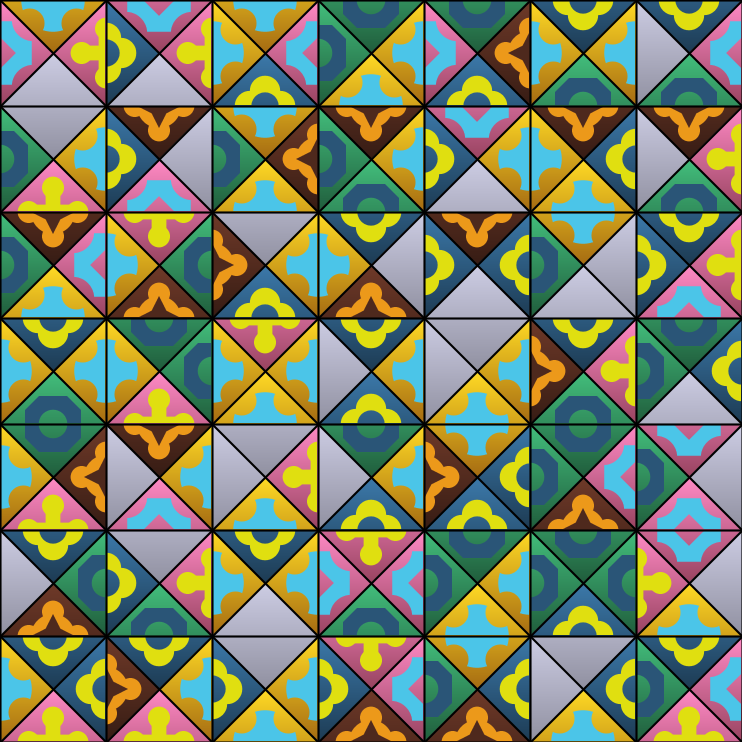
\includegraphics[width=45mm]{images/shuffled.png}}
  \hspace{5mm}
  \subfloat[Solved]{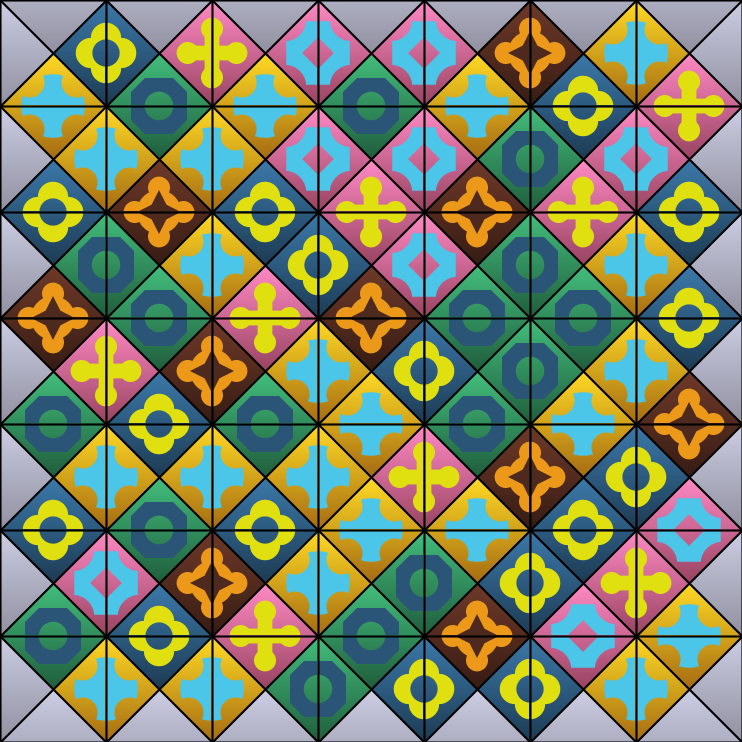
\includegraphics[width=45mm]{images/solved.png}}
  \caption{Simplified puzzle with 7 by 7 tiles, with 6 patterns}
  \label{fig:7x7_example}
\end{figure}

Each piece has its edges marked with different shape and colour combinations, henceforth called patterns. Each must precisely match the neighboring piece's edge when the puzzle is solved. These pieces can also be placed in four different positions, by rotating them 90º, 180º or 270º. Pieces that will sit on a corner or borderline tile can be easily distinguished from all the other, as they have a grey edge. There are 22 different patterns in the original puzzle (excluding the grey edges).

\subsection{Normal approaches to solving the problem}\label{sec:normal_approaches}

We have found that the most common approaches that solve these kinds of problems falls into one of two types: swap and iterative. Swap solutions always start with a complete board, and then use the rotate and swap operations in order to improve the board's state. Iterative approaches place pieces progressively, according to a certain criteria and can backtrack to any previous state if they determine that no good solution will be found from that point onward.

\subsubsection{The swap approach}\label{sec:swap_approach}

As said before, swap approaches begin by placing all the available pieces in the board, then use the swap and rotate operations to improve the board's state. There are plenty algorithms that can achieve this, like hill-climbing, tabu search and simulated annealing. These approaches evaluate the board's state and try to find which sequence of operations will achieve the greatest score possible (which in turn will lead to a solved puzzle).

Evidently, the starting position of the pieces in the puzzle will also play an important part on the rest of the solving process. (Explain why?)

\subsubsection{The iterative approach}\label{sec:iterative_approach}

Iterative solutions try to place the pieces progressively, usually following some kind of pattern.
(Describe here most common patterns that can be used.)

\section{Solving Eternity II with Genetic Algorithms}\label{sec:genetic_algorithms}

\subsection{Genetic Algorithms}

%(Methodologies and approaches taken when trying new methods to improve solving times of The desired simplified Eternity II puzzles)

A genetic algorithm is an informed search method that mimics the process of natural evolution. It is particularly useful in search and optimization problems.

The genetic algorithm works by generating solutions using procedures inspired by natural evolution: the search process begins with a set, called \textit{population} of initial states, called \textit{individuals or chromosomes}. The characteristics that make up each individual can therefore be thought of as \textit{genetic material}. The quality of the solution each individual represents is measured by a problem-specific \textit{fitness} function. Evolution of the population (and consequently of the best solution) is achieved by \textit{selection} and \textit{reproduction} between individuals of the population, often in some respect to their fitness evaluation. This creates new individuals in the population whose genetic material comes from individuals in the previous generation.\cite{peck_dhawan}

\textit{Mutations} in the individuals are often introduced between generations so that we can diverge from the set that contains all possible combinations of genetic material present in the initial population, which may or may not include the solution or optimization sought after.

These kind of algorithms have been proven useful in solving many kinds of problems, including puzzle problems. A textbook example of successful application of genetic algorithms in puzzle-solving problems is the \textit{n-queens} problem\cite{eastridge}.

\subsection{Methodology}\label{sec:methodology}

\subsubsection{Chromosomes and genetic material}

A key step of solving problems with genetic algorithms is defining the structure of an individual. Textbook examples of genetic algorithms often use individuals represented by structures as simple as bit strings or natural number arrays. For this particular application of genetic algorithms we consider that there is no advantage in encoding the board state in a bit string or number array. Therefore, we chose to use the most direct representation of a board state available to us.

The genetic material present in each chromosome is, therefore, the position and rotation of each one of the pieces present in the board. Clusters of pieces that appear to be correctly placed on the board are the traits we want to pass on to future generations. We refer to these as \textbf{features}.



\subsubsection{Initial state and population}

The initial state in our search problem is the board we want to solve. It defines the unique characteristics of the problem: the problem size and the set of pieces that will be present in all individuals of the population.

The initial population of $n$ individuals is built by randomly shuffling the original board $n$ times.

\subsubsection{Fitness function}\label{sec:fitness-function}

The fitness function used to evaluate the quality of the boards is given by:

\begin{figure}[H]
  \begin{equation}
    fitness = \frac{n\_matching\_edges}{total\_matching\_edges}
  \end{equation}
  \caption{Fitness function for evaluating boards}
  \label{fig:eq:fitness_function}
\end{figure}

where \textit{n\_matching\_edges} represents the number of matching edges between all pieces of the board for the current state, and \textit{total\_matching\_edges} the number of matching edges for an $n*n$ board. As such, \textit{fitness} will yield a value between $[0.0, 1.0]$, with higher values corresponding to fitter boards. A fitness of exactly $1.0$ would only be attributed to a board that is correctly solved.

The number of matching grey edges (correctly placed on the borders) is also accounted for in our fitness function.

\subsubsection{Breeding}

Starting out with $n$ random permutations of the same board, the fittest half of the population is selected for breeding, using an elitist selection approach with stochastic breeding. These specimens are then bred and their genetic code is crossed-over according to very specific rules:

\begin{itemize}
  \item If both parents have compatible features, use both features on both descendants in order to create fitter boards
  \item If both parents have incompatible features, select the highest scoring feature from each parent and use it as a starting point for each of the descendants
  \item The rest of the genetic code (pieces) not originated from the feature selection is then placed on the descendant boards using a simple (no backtracking) linear constructive method
  \item Mutations are then performed on a random set of pieces by rotating them in order to try and improve the overall fitness of the board
\end{itemize}

\subsubsection{Mutations}\label{sec:mutations}

After each reproduction each new individual suffers a series of mutations (with a probability of 50\%). These mutations are piece-oriented, and are performed by selecting $n-1$ random pieces (where $n$ corresponds to the size of the board) and rotating them clockwise. This approach provides solid results, until the board score nears its maximum: when this situation arises, the solution becomes stagnant due to the fact that only one or two pieces need to be rotated to achieve a correct solution. To overcome this problem, when the board score reaches a certain threshold ($score >= maximum score - 4$), all board pieces are checked and rotated (if necessary), in order to maximize the number of connections, providing a correct solution in most observed cases.

\subsection{Implementation}\label{sec:implementation}

\subsubsection{State representation}\label{sec:state_representation}

The two dimensional \textit{board} structure is internally represented as a single dimension array of \textit{piece} structures together with the value of the board's width (or height). Accessing the board with the two dimensional argument ($column$, $row$) is therefore equivalent to writing the one dimensional argument ($column + width * row$).


\subsubsection{Feature Extraction}\label{sec:feature_extraction}

Extracting features from the board was achieved by developing a recursive strategy, as described in Appendix A.%\nameref{sec:feature_extraction}.

\subsubsection{Eternity II Editor}\label{sec:eternity2_editor}

(Why are we using Eternity II Editor and how we linked the previously developed solution with it)

\section{Results}\label{sec:results}

This implementation lead to good experimental results, being able to successfully complete boards up to 10x10 in size.

\subsection{Population Size}\label{sec:population_size}

By testing different configurations of the population size it was determined the minimum and most effective number for the initial population was eight elements, as Fig. \ref{fig:population_stats} shows.

\begin{figure}[H]
  \centering
  \subfloat[Iterations]{\label{fig:pop_iterations}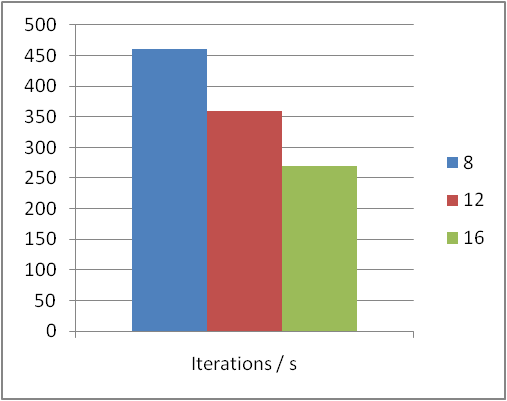
\includegraphics[width=40mm]{images/pop_iterations.png}}
  \subfloat[Iterations / s]{\label{fig:pop_iterations_sec}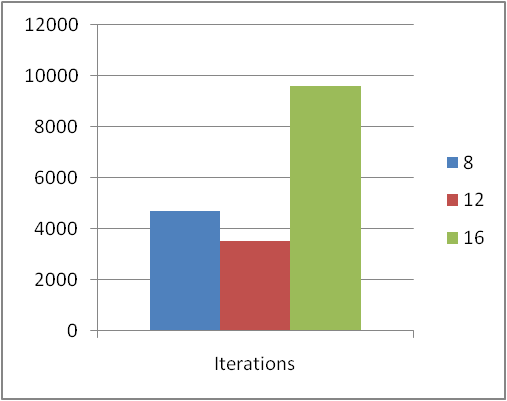
\includegraphics[width=40mm]{images/pop_iterations_sec.png}}
  \subfloat[Time (secs)]{\label{fig:pop_time}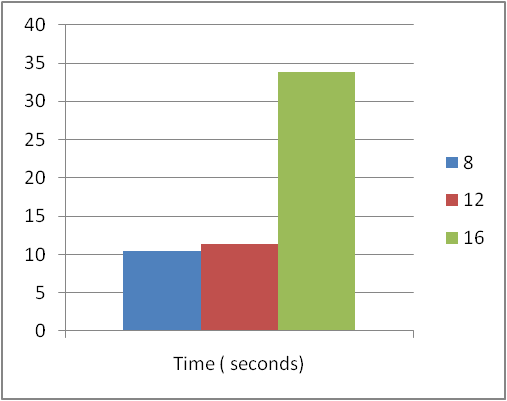
\includegraphics[width=40mm]{images/pop_time.png}}
  \caption{Initial population tests with a board with 7 by 7 tiles, 6 patterns}
  \label{fig:population_stats}
\end{figure}

These results were obtained by solving the 7x7x6 board five consecutive times, using different values for the population size (eight, twelve and sixteen, respectively). It is clear that, in this implementation, a smaller number for the population leads to better results, not requiring as many iterations (and therefore less time) to reach a valid solution.

\subsection{Fitness Evolution}\label{sec:fitness_evolution}

\begin{figure}[H]
  \centering
  \subfloat[7x7]{\label{fig:fitness_evolution_7x7}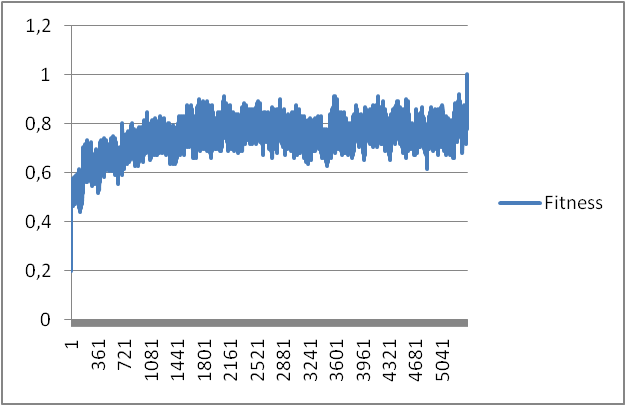
\includegraphics[width=70mm]{images/fitness_evolution_7x7.png}}
  \subfloat[10x10]{\label{fig:fitness_evolution_10x10}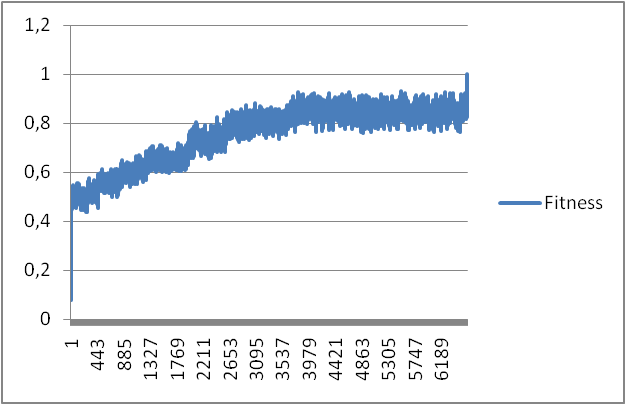
\includegraphics[width=70mm]{images/fitness_evolution_10x10.png}}
  \hspace{40mm}
  \subfloat[11x11]{\label{fig:fitness_evolution_11x11}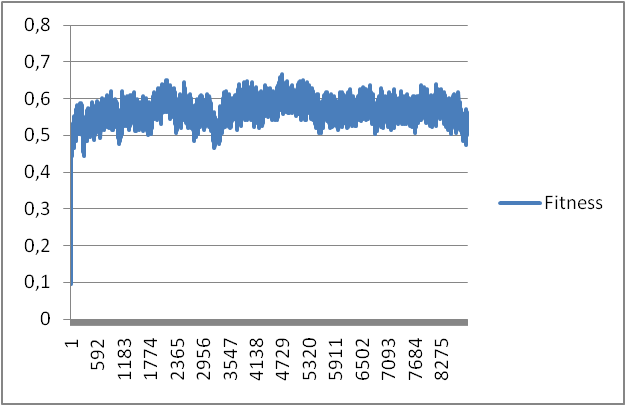
\includegraphics[width=70mm]{images/fitness_evolution_11x11.png}}
  \caption{Initial population tests with a board with 7 by 7 tiles, 6 patterns}
  \label{fig:population_stats}
\end{figure}

\section{Conclusions}\label{sec:conclusions}

Although we found moderate success in solving the puzzles presented in the section X: Results  (referir?), our solution proved unfeasible when trying to solve puzzles of greater dimensions (like those in a 11x11 board). One might argue that Genetic Algorithms are better at optimizing solutions than they are at finding a particular one.

In fact, the evaluation that the fitness function continually does not always point in the direction of the solution sought after, as we may reach a state where the population has a high average fitness value, appearing to be closer to the solution, when in fact it is not.

Our feature extraction procedure is to blame here. Bigger features contribute more to the feature evaluation, and it's very difficult for th

\subsection{Future Work}
% ---- Bibliography ----
\bibliographystyle{plain}
\bibliography{mpes}

\newpage

%\section*{Appendix A: feature extraction}\label{sec:app:feature_extraction}

\begin{algorithm}
\caption{feature extraction algorithm}
\label{feature extraction algorithm}
\newcommand{\algorithmicfunction}{\textbf{function}\ }
\newcommand{\logicaland}{\textbf{and}\ }
  \begin{algorithmic}

  \STATE \algorithmicfunction getfeatures() :

  \STATE $visited \gets empty set$
  \STATE $features \gets empty list$
  \STATE $n_{squares} \gets problem size$

  \FOR{$i \gets 1$ to $n_{squares}$}
    \IF{$i$ is not in $visited$}
      \STATE $newfeature \gets empty board$
      \STATE recursefeatures($i$, $feature$, $visited$)
      \STATE append $newfeature$ to $features$
    \ENDIF
  \ENDFOR
  \RETURN $features$
  \end{algorithmic}

  \begin{algorithmic}
  \STATE \algorithmicfunction recursefeatures($i$, $feature$, $visited$) :
    \STATE $currentpiece \gets board[i]$
    \STATE $feature[i] \gets currentPiece$
    \FOR{$direction$ in $north$, $east$, $south$, $west$}
      \STATE $neighbour \gets$ getneighbour($i$, $direction$)
      \STATE $neighbourindex \gets$ getneighbourindex($i$, $direction$)
      \IF{$neighbour$ exists
      \logicaland $feature[i]$ is empty \logicaland $neighbourindex$ not in $visited$}
        \STATE $oppositedirection \gets$ getoppositedirection($direction$)
        \IF{getpattern($currentpiece$, $direction$) matches getpattern($neighbour$, $oppositedirection$))}
          \STATE{recursefeatures($neighbourindex$, $feature$, $visited$)}
        \ENDIF
      \ENDIF
    \ENDFOR
  \end{algorithmic}
\end{algorithm}

\end{document}

